\documentclass[a4paper,12pt]{report}
\usepackage[utf8]{inputenc}
\usepackage[italian]{babel}
\usepackage[hidelinks]{hyperref}
\usepackage{graphicx}
\usepackage{caption}
\usepackage{lmodern}
\usepackage{setspace}
\usepackage{geometry}
\usepackage{titlesec}
\usepackage{fancyhdr}
\usepackage{tocloft}
\usepackage{etoolbox}
\geometry{margin=2cm}

% Numerazione sezioni e sottosezioni
\renewcommand{\thesection}{\thechapter.\arabic{section}}
\renewcommand{\thesubsection}{\thesection.\arabic{subsection}}
\setcounter{secnumdepth}{2}
\setcounter{tocdepth}{2}

% Font per sezioni
\titleformat{\section}
  {\normalfont\small\bfseries}
  {\thesection}{1em}{}

\titleformat{\subsection}
  {\normalfont\small\itshape}
  {\thesubsection}{1em}{}



%impostazione personalizzate per linee di codice
\usepackage{listings}
\usepackage[x11names]{xcolor}
\definecolor{MyGreen}{HTML}{16610E}

\lstset{
  basicstyle=\ttfamily\footnotesize,
  breaklines=true,
  breakatwhitespace=true,
  keywordstyle=\color{blue},
  commentstyle=\color{gray},
  stringstyle=\color{MyGreen},
  showstringspaces=false,
  columns=fullflexible,
  language=Python
}

% Impostazioni personalizzate per capitoli e piè di pagina
\titleformat{\chapter}[block]
  {\normalfont\Huge\bfseries}
  {\relax} % rimuove "Capitolo N"
  {0pt}
  {}

\pagestyle{fancy}
\fancyhf{}
\fancyfoot[C]{Capitolo \thechapter\ -- \thepage}


\begin{document}

% --- Copertina ---
\begin{titlepage}
    \begin{center}
        
\includegraphics[width=0.4\textwidth]{logo-universita.png}
        \Large\textbf{UNIVERSIT\`A DEGLI STUDI DI CATANIA}\\[0.3cm]
        \large Dipartimento di Matematica e Informatica\\
        \large Corso di Laurea Triennale in Informatica\\[2cm]

        \vspace{2cm}

        {\Huge \textbf{VolleyLive}}\\[0.5cm]
        {\large Sistema di monitoraggio, analisi e visualizzazione\\
        delle partite di pallavolo in tempo reale}\\[2.5cm]

        \vspace{1cm}

        \begin{flushleft}
            \textbf{Studente:} \\
            Claudio Nuncibello
        \end{flushleft}

        \vspace{1cm}

        \begin{flushright}
            \textbf{Relatore:} \\
            Prof. Salvatore Nicotra
        \end{flushright}

        \vfill

        \textbf{Anno Accademico 2024/2025}
    \end{center}
\end{titlepage}

% --- Abstract e logo ---
\newpage
\thispagestyle{empty}
\vspace*{2cm}
\begin{center}
    
\includegraphics[width=0.4\textwidth]{volleylive-logo.png} \\[1.5cm]
    \textbf{\LARGE Abstract} \\[1cm]
    \begin{minipage}{0.85\textwidth}
        \small
        Il progetto VolleyLive nasce con l’obiettivo di monitorare e analizzare in tempo reale le partite di pallavolo, combinando tecnologie moderne per la gestione dei dati in streaming e la visualizzazione interattiva. Il sistema raccoglie snapshot live da API sportive, li trasforma e li distribuisce tramite una pipeline composta da Kafka, Logstash, Spark ed Elasticsearch. I dati vengono visualizzati in una dashboard frontend sviluppata in Next.js, offrendo funzionalit\`a come la selezione dei match preferiti e l’analisi predittiva dell’esito delle partite. L’intero progetto \`e containerizzato tramite Docker e supporta l’estensibilit\`a verso nuovi modelli e sport. Questa tesi descrive l’architettura, le scelte progettuali, e i risultati ottenuti attraverso l’implementazione del sistema.
    \end{minipage}
\end{center}
\newpage

% --- Indice ---
\tableofcontents
\newpage

% ===============================
% INTRODUZIONE
% ===============================
\chapter*{Introduzione}
\addtocontents{toc}{\vspace{0.3cm}\textbf{Introduzione}\par}

Il presente elaborato descrive lo sviluppo di VolleyLive: un sistema per il monitoraggio e l’analisi in tempo reale delle partite di pallavolo. Il progetto nasce nell’ambito dell’analisi sportiva, oggi in profonda trasformazione, favorita dalla crescente disponibilità di dati e dall’utilizzo di tecnologie per l’elaborazione in streaming. L’integrazione di API sportive, strumenti di monitoraggio e algoritmi analitici consente oggi non solo di osservare lo svolgimento di una competizione, ma anche di interpretarne dinamicamente l’andamento e prevederne l’evoluzione. L’analisi in tempo reale ha assunto un ruolo centrale in numerosi ambiti applicativi, dallo sport professionale alla logistica industriale. Nel mondo sportivo tuttavia strumenti avanzati di elaborazione live sono spesso riservati a discipline molto seguite (come calcio o basket), o a contesti professionali ad alto budget. Per molte altre discipline come la pallavolo esistono margini significativi per migliorare l’accessibilità e la fruibilità dei dati durante gli eventi. VolleyLive non si propone soltanto come una soluzione funzionale per il monitoraggio in tempo reale, ma getta le basi per un sistema estensibile e orientato al futuro delle competizioni sportive. Grazie all’adozione di tecnologie scalabili e open source, la piattaforma si presta a essere ampliata per integrare nuove fonti dati e modelli predittivi sempre più sofisticati. In questo senso, VolleyLive rappresenta una prima esplorazione concreta verso sistemi intelligenti di supporto all’analisi sportiva, potenzialmente applicabili non solo alla pallavolo ma a molte altre discipline. Il sistema adotta tecnologie all'avanguardia come Kafka per la gestione del flusso dati, Logstash per la trasformazione degli eventi, Spark per l’elaborazione in tempo reale, Elasticsearch per l’indicizzazione e la consultazione, e una web app per la visualizzazione lato utente. Il tutto è orchestrato tramite container Docker, in modo da garantire portabilità, isolamento e semplicità di gestione. Gli obiettivi principali del progetto sono: costruire una pipeline dati solida e scalabile, in grado di gestire flussi continui di snapshot aggiornati ogni dieci secondi; applicare modelli di analisi per stimare in tempo reale l’esito delle partite in corso; offrire un’interfaccia intuitiva e interattiva per la consultazione live dei match; garantire la tracciabilità storica dei dati raccolti, utile per analisi retrospettive e sviluppo futuro di modelli predittivi più avanzati. Dal punto di vista applicativo, VolleyLive è pensato per essere utilizzato sia da utenti generici interessati a seguire una competizione sia da figure più tecniche come data analyst sportivi o scout, che necessitano di uno strumento semplice e flessibile per leggere, filtrare e confrontare partite in tempo reale. L'elaborato è articolato in cinque capitoli: nel capitolo primo capitolo si descriverà l’architettura generale del sistema e i componenti principali, soffermandosi sulle tecnologie adottate e sul loro ruolo nella pipeline; il secondo capitolo approfondirà il funzionamento della raccolta dati live tramite API e il terzo illustra i meccanismi di ingestione, trasformazione ed elaborazione in streaming; il quarto capitolo è dedicato alla visualizzazione e all’interazione tramite dashboard web; Il quinto capitolo presenta una serie di risultati ottenuti attraverso l’esecuzione del sistema, evidenziando esempi pratici e scenari d’uso. Nelle conclusioni sono raccolte le riflessioni conclusive e si suggeriscono direzioni per futuri sviluppi ed estensioni. VolleyLive si propone quindi come una base concreta per sperimentare tecnologie moderne per lo streaming e l’analisi dei dati sportivi, ponendo particolare attenzione all’affidabilità del flusso, alla chiarezza della visualizzazione e alla possibilità di estensione verso altri sport o contesti analitici.

% ===============================
% CAPITOLO 1 - Architettura
% ===============================

\chapter{Architettura Generale del Sistema}

Il sistema VolleyLive è stato concepito e realizzato seguendo un approccio modulare e scalabile, con l’obiettivo di garantire affidabilità, continuità del flusso dati e facilità di estensione. Questo capitolo descrive nel dettaglio l’architettura generale adottata, soffermandosi su ciascuna delle tecnologie impiegate, sul ruolo che ricoprono nella pipeline e sulle relazioni tra i vari moduli.


\section{Panoramica dei Componenti Tecnologici}

Iniziamo con il dare una descrizione dettagliata dei principali componenti tecnologici che costituiscono il sistema VolleyLive, evidenziando il ruolo operativo di ciascun modulo all’interno della pipeline. Ogni tecnologia è presentata nel contesto del suo impiego pratico, illustrandone le funzionalità chiave e le modalità con cui interagisce con gli altri elementi del sistema.


\subsection{Fonte Dati: SportDevs API}

Il sistema VolleyLive si basa sui dati forniti dalle API pubbliche di SportDevs, che rappresentano la fonte principale per l’acquisizione delle informazioni relative alle partite in corso. Queste API espongono una serie di endpoint REST, interrogabili in formato \texttt{JSON}, attraverso cui è possibile ottenere dati grezzi aggiornati sulle partite live. A partire dagli endpoint il sistema costruisce, tramite successive trasformazioni, snapshot strutturati e coerenti, idonei a essere impiegati nei modelli di previsione.

Nel flusso di sistema le API costituiscono il punto iniziale della pipeline, i dati vengono estratti regolarmente dallo script \textit{producer} che li interroga ogni dieci secondi. I dati ricevuti vengono poi normalizzati e strutturati per essere inoltrati a Kafka nel formato previsto. L'accesso avviene tramite chiave API e richiede attenzione nella gestione della frequenza di interrogazione per evitare di superare i limiti imposti dal servizio.

Nonostante l’ampia copertura e il buon livello di dettaglio, le API presentano però alcune limitazioni. In particolare, durante le partite di campionati minori si riscontrano occasionali ritardi nell’aggiornamento dei punteggi, e la gestione del set di \textit{tiebreak} può risultare imprecisa o mancante. Queste problematiche sono note e, al momento, vengono gestite a livello applicativo convivendo con le possibili incongruenze nel dato.

Nel complesso, SportDevs rappresenta una soluzione efficace per alimentare in tempo reale il sistema VolleyLive, pur richiedendo l’adozione di logiche resilienti in fase di raccolta e validazione dei dati.

\subsection{Elaborazione e Normalizzazione: Logstash}

Logstash è il primo componente della pipeline incaricato della trasformazione dei dati in arrivo dalle API di VolleyLive. Riceve direttamente i dati grezzi forniti dallo script Python (producer), li interpreta e li converte in un formato strutturato, adatto alla successiva pubblicazione su Kafka.

Le operazioni svolte da Logstash includono la normalizzazione dei nomi dei campi, l’estrazione di \textit{timestamp} coerenti, la gestione di dati opzionali o incoerenti, e l’aggiunta di metadati utili (come gli identificativi univoci del match). Queste trasformazioni avvengono tramite pipeline configurabili in formato dichiarativo, che permettono di adattare con facilità le regole di parsing e filtraggio.

Una volta completata l’elaborazione, Logstash pubblica gli \textit{snapshot} trasformati su un \textit{topic} Kafka, rendendoli disponibili per le successive fasi di analisi e indicizzazione. In questo modo, Logstash funge da punto di ingresso intelligente per il flusso dati del sistema, garantendo uniformità e qualità nella base informativa di VolleyLive.


\subsection{Gestione del Flusso Dati: Kafka}

Kafka è il sistema di messaggistica distribuito adottato da VolleyLive per la gestione affidabile e scalabile del flusso dati in tempo reale. All’interno dell’architettura, Kafka riceve i dati già trasformati da Logstash e li rende disponibili per i successivi moduli di analisi e indicizzazione.

Ogni snapshot elaborato viene pubblicato su un \textit{topic} Kafka, da cui può essere consumato in parallelo da più servizi, come Apache Spark o eventuali altri moduli analitici. Questo modello basato su pubblicazione e sottoscrizione (\textit{pub/sub}) consente un’elaborazione asincrona, modulare e facilmente estendibile.

La scelta di utilizzare Kafka è stata motivata dalla necessità di gestire un flusso continuo di eventi con frequenti aggiornamenti, mantenendo elevate garanzie di durabilità, ordinamento e possibilità di \textit{replay} dei messaggi. La sua architettura nativamente distribuita lo rende particolarmente adatto a scenari \textit{real-time} come quello di VolleyLive.


\subsection{Analisi Streaming: Apache Spark}

Apache Spark è il componente dedicato all’elaborazione avanzata dei dati in streaming nel sistema VolleyLive. Dopo che gli \textit{snapshot} sono stati pubblicati su Kafka da Logstash, Spark li consuma in tempo reale per applicare logiche analitiche e generare output destinati all’indicizzazione.

L’implementazione sfrutta Spark Structured Streaming, un sistema che elabora i dati in tempo reale suddividendoli in piccoli blocchi temporali (\textit{micro-batch}). Anche se i dati arrivano in modo continuo, Spark li raggruppa ogni pochi secondi e li processa in modo ordinato e affidabile. Questo approccio garantisce una \textit{semantica end-to-end}, ossia l’elaborazione completa, senza perdite o duplicazioni, di ogni blocco di dati dall’ingresso all’output finale.

Nel contesto di VolleyLive, Spark viene utilizzato per applicare filtri, trasformazioni strutturali e, in prospettiva, funzioni di analisi predittiva basate su modelli di \textit{machine learning}.

Spark si colloca tra la distribuzione dei dati (Kafka) e la fase di visualizzazione (Elasticsearch), fungendo da nodo di elaborazione intermedio. Questa configurazione permette di isolare la logica analitica dal resto della pipeline, semplificando l’estensione futura del sistema verso algoritmi più sofisticati.


\subsection{Indicizzazione e Ricerca: Elasticsearch}

Elasticsearch è il motore di ricerca e indicizzazione adottato nel sistema VolleyLive per rendere interrogabili e visualizzabili gli \textit{snapshot} elaborati in tempo reale. Dopo l’elaborazione su Apache Spark, ogni snapshot viene inviato a Elasticsearch, dove viene memorizzato come documento JSON strutturato.

Tutti i dati, inclusi gli score predittivi e le informazioni live, vengono inseriti all’interno di un unico indice. Questa scelta progettuale consente di ottenere, tramite una singola query, tutte le informazioni aggiornate relative a un match, semplificando l’accesso lato frontend e migliorando l’efficienza delle chiamate.

L’indice è configurato con un \textit{mapping} coerente, che definisce esplicitamente la struttura e i tipi dei campi per garantire interrogazioni affidabili e prestazioni ottimali. Questo approccio assicura una base dati consistente e facilmente estendibile anche in fase di evoluzione del sistema.

Infine, per attività di \textit{debugging}, monitoraggio e ispezione manuale dei dati, il sistema fa uso di Kibana, uno strumento di visualizzazione integrato con Elasticsearch, utile in particolare durante le fasi di sviluppo.


\subsection{Visualizzazione: Frontend React/Next.js}

L’interfaccia utente di VolleyLive è sviluppata utilizzando il framework React in combinazione con Next.js, una soluzione moderna e performante per la realizzazione di applicazioni web dinamiche. Il frontend fornisce agli utenti una dashboard interattiva e reattiva per consultare lo stato in tempo reale delle partite, visualizzare punteggi, set e score predittivi.

Per accedere ai dati, il frontend comunica con un backend intermedio realizzato in FastAPI. Questo backend funge da strato di accesso alle informazioni archiviate in Elasticsearch, esponendo API REST personalizzate per effettuare query sui match live. Tale approccio consente di mantenere il database isolato, migliorare la sicurezza e semplificare la gestione delle richieste dal lato client.

La struttura della dashboard permette agli utenti di selezionare match preferiti live e visualizzare in dettaglio l’andamento di ciascun incontro. L’interfaccia è stata progettata per adattarsi ai diversi dispositivi.

Il frontend è containerizzato e integrato nell’infrastruttura tramite Docker, in modo da garantire coerenza tra ambiente di sviluppo e produzione e facilitare il deployment del sistema completo.


\subsection{Containerizzazione: Docker e Visualizzazione dell’Architettura}

Il sistema VolleyLive adotta una configurazione interamente containerizzata, implementata tramite Docker, al fine di garantire portabilità, isolamento e semplicità di gestione in tutte le fasi del ciclo di vita dell’applicazione. Ogni componente è incapsulato in un container indipendente, facilitando la manutenzione, il testing e il deployment multiambiente.

L’infrastruttura è orchestrata mediante \texttt{docker-compose}, che consente di avviare l’intero ecosistema tramite un’unica configurazione centralizzata. I servizi comunicano all’interno di una rete virtuale definita da Docker, riducendo le dipendenze esterne e i problemi di configurazione ambientale.

Tutti i moduli descritti nei paragrafi precedenti – inclusi il \textit{producer} Python, i servizi di elaborazione e analisi, l’API backend e l’interfaccia web – sono containerizzati e integrati nell’infrastruttura, assicurando coerenza tra ambiente di sviluppo e produzione.

Lo schema architetturale riportato in Figura~\ref{fig:architettura} illustra il flusso dei dati e le interazioni principali tra i servizi, dalla raccolta degli snapshot fino alla visualizzazione finale.

\begin{figure}[ht]
    \centering
    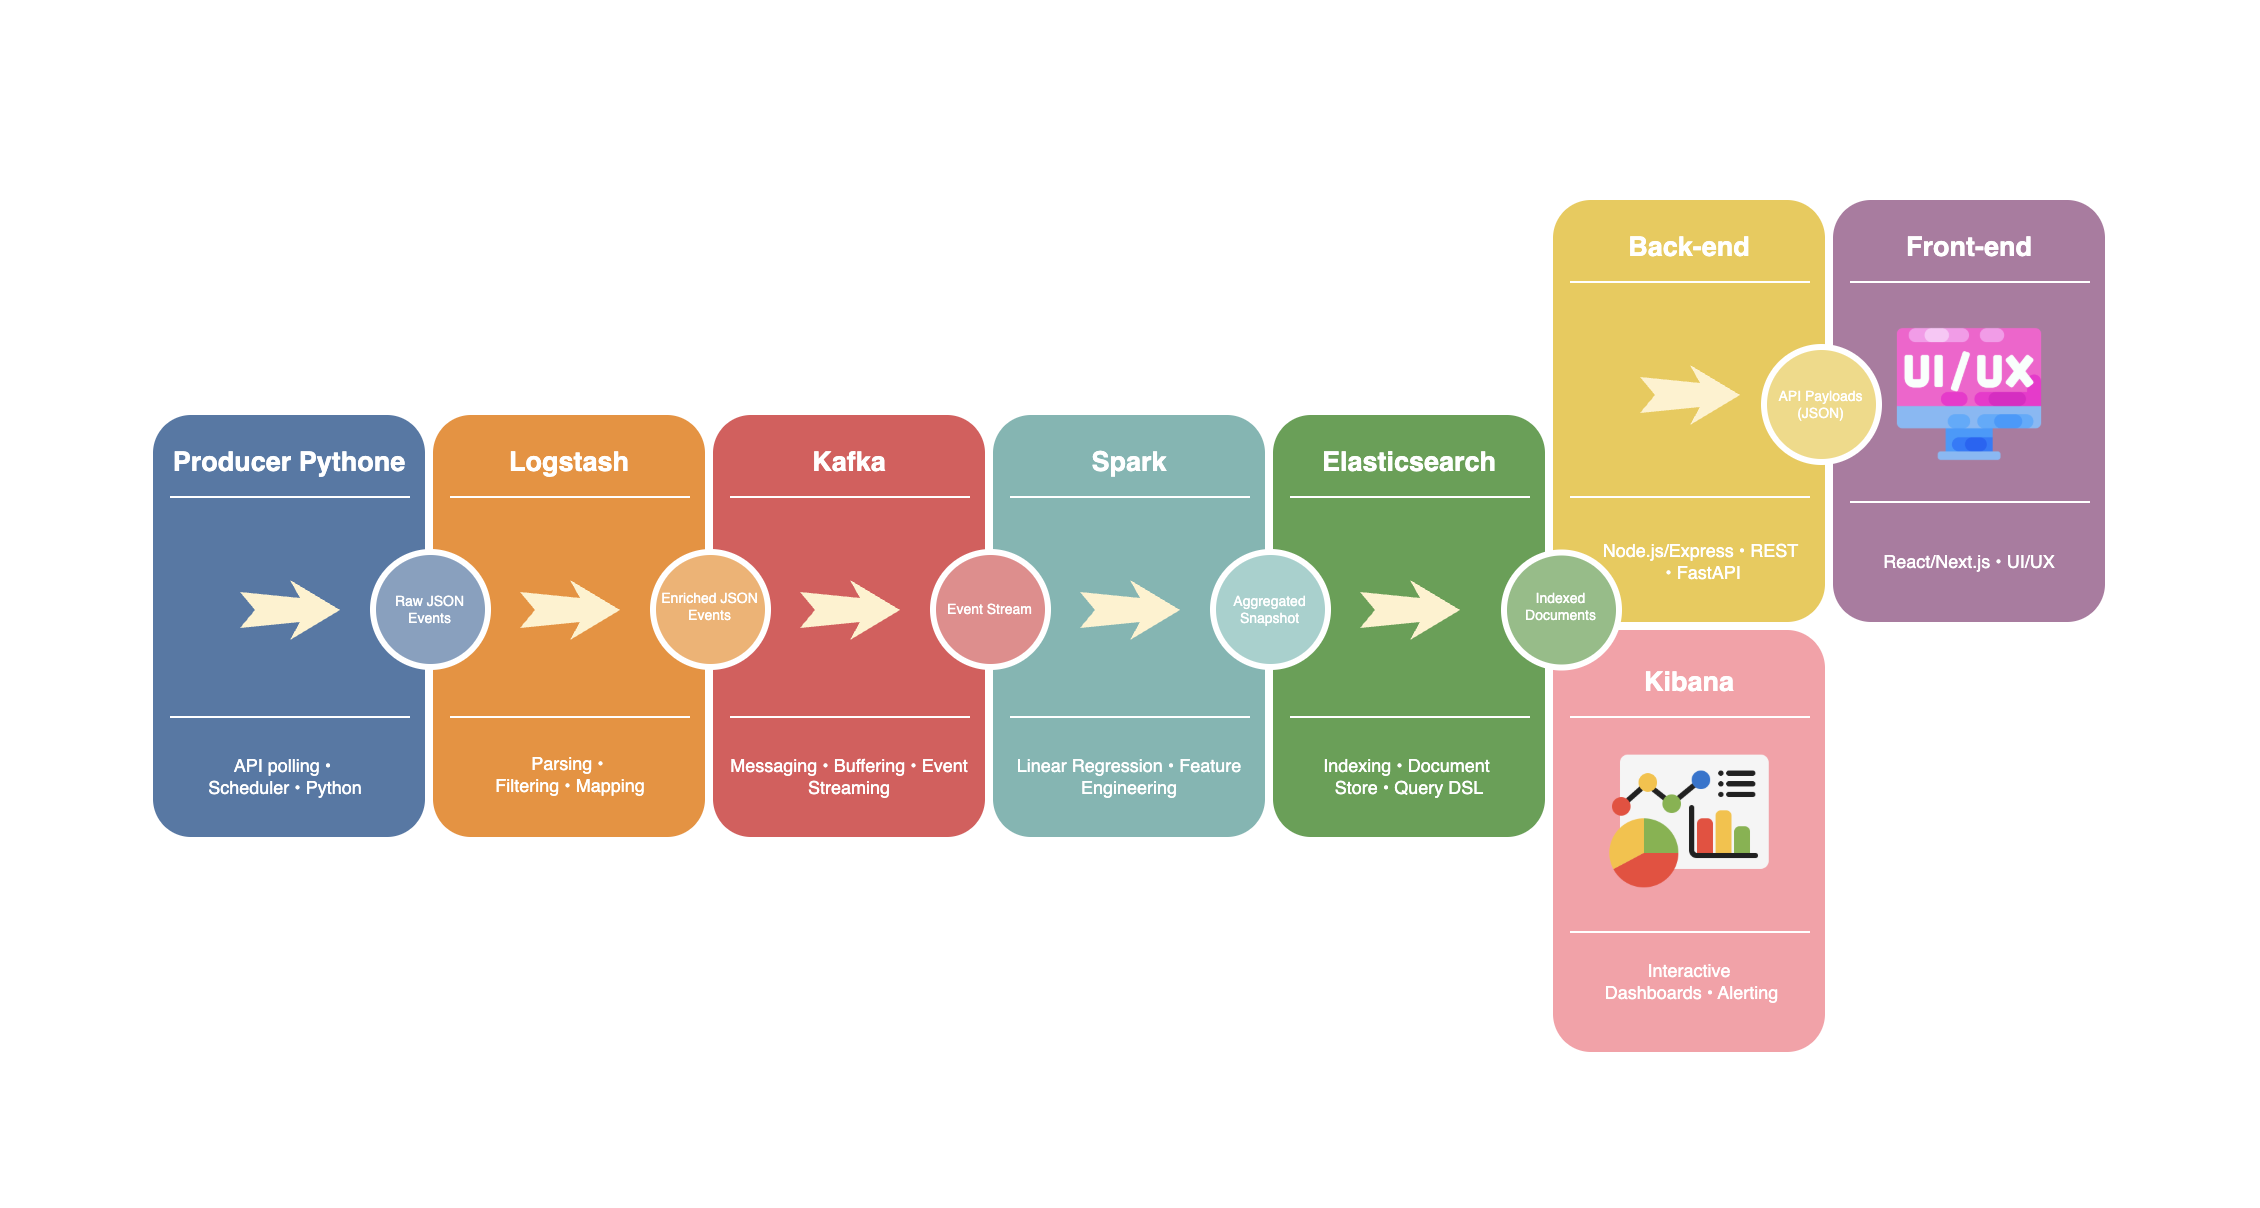
\includegraphics[width=0.9\textwidth]{schema-architettura.png}
    \caption{Architettura containerizzata del sistema VolleyLive}
    \label{fig:architettura}
\end{figure}


\section{Scelte Progettuali e Motivazioni}

La definizione dell’architettura di VolleyLive è frutto di un processo decisionale che ha bilanciato esigenze di efficienza, semplicità operativa e finalità analitiche.
In questa sezione vengono descritte le principali alternative valutate e le motivazioni che hanno portato alla definizione dell’architettura presentata nel paragrafo precedente.

\subsection{Pipeline Always-On vs On-Demand: Analisi Comparativa}

Nel progettare il sistema VolleyLive, si è valutata la possibilità di attivare la pipeline dati solo in risposta a un’azione dell’utente (approccio \textit{on-demand}) oppure di mantenerla costantemente attiva (approccio \textit{always-on}). La modalità \textit{on-demand}, sebbene più leggera dal punto di vista computazionale, avrebbe comportato una latenza iniziale, una complessità maggiore nel coordinamento tra moduli e una perdita della continuità storica. L’approccio \textit{always-on} garantisce invece un flusso costante e affidabile di dati, semplificando il design complessivo e consentendo l’elaborazione in tempo reale anche in assenza di richieste attive.

\subsection{Motivazioni della Scelta dell’Architettura Always-On}

L’adozione dell’architettura \textit{always-on} è stata guidata da due esigenze fondamentali: da un lato, garantire l’affidabilità e la continuità del flusso dati; dall’altro, costruire una base dati storica che consenta analisi retrospettive e l’applicazione di modelli predittivi. Inoltre, la natura del progetto – focalizzato sull’utilizzo di tecnologie di data streaming e containerizzazione – trova piena espressione in un sistema sempre attivo, che riflette in modo coerente gli obiettivi sperimentali della tesi.


% ===============================
% CAPITOLO 2 - Pipeline dei Dati Live
% ===============================

\chapter{Acquisizione e Gestione dei Dati in Real-Time}

In questo capitolo viene descritta la prima parte della pipeline utilizzata da VolleyLive, dedicata alla raccolta e alla gestione iniziale dei dati provenienti da partite di pallavolo in corso. Il focus sarà sulle tecnologie e le metodologie impiegate per acquisire dati live, trasformarli in un formato standardizzato e distribuirli attraverso un flusso dati affidabile e scalabile.

I paragrafi di questo capitolo affrontano in maniera approfondita ciascuno dei passaggi fondamentali: dall'acquisizione iniziale tramite script Python, alla normalizzazione effettuata da Logstash, fino alla distribuzione tramite Kafka. Ogni fase sarà illustrata nel dettaglio, sottolineando le scelte tecniche effettuate e le loro motivazioni.

\section{Acquisizione Dati: Producer Python}

\subsection{Introduzione agli Snapshot Live}

Nella pipeline dati del progetto VolleyLive, lo snapshot live rappresenta il punto iniziale e fondamentale per ogni successiva elaborazione ed analisi. Per snapshot si intende una fotografia periodica e dettagliata dello stato corrente di ciascuna partita monitorata. Tali istantanee sono catturate a intervalli temporali regolari (ogni pochi secondi), al fine di garantire una visione costantemente aggiornata degli eventi sportivi in corso.

L’impiego degli snapshot live si rivela cruciale poiché essi costituiscono non solo la base per l’analisi in tempo reale, ma anche una risorsa fondamentale per alimentare il dataset storico, contribuendo così a migliorare nel tempo l’accuratezza delle predizioni effettuate dal sistema.


\subsection{API SportDevs: Dati e Endpoint Utilizzati}

La raccolta dei dati live viene effettuata interrogando direttamente le API pubbliche di SportDevs, che permettono di accedere a informazioni aggiornate in tempo reale sulle partite di pallavolo. Queste API restituiscono dati in formato JSON, facilmente integrabili all'interno del sistema VolleyLive.
Il producer Python utilizza principalmente tre endpoint. Il primo è:

\url{https://volleyball.sportdevs.com/matches?status_type=eq.live}

Questo endpoint restituisce tutte le partite attualmente in corso e fornisce i dati essenziali per comporre uno snapshot live, come il punteggio per ciascun set, lo stato della partita, gli ID delle squadre coinvolte e altre informazioni contestuali.
Il secondo endpoint utilizzato è:

\url{https://volleyball.sportdevs.com/matches?or=(home_team_id.eq.{team_id},away_team_id.eq.{team_id})&order=specific_start_time.desc&limit=5}

Questo viene impiegato per ottenere gli ultimi cinque incontri disputati da una specifica squadra, identificata dal parametro \texttt{team\_id}. Tali informazioni possono essere utilizzate per arricchire gli snapshot con contesto storico immediato.
Infine, il terzo endpoint è:

\url{https://volleyball.sportdevs.com/matches?or=(and(home_team_id.eq.{home_id},away_team_id.eq.{away_id}),and(home_team_id.eq.{away_id},away_team_id.eq.{home_id}))&order=specific_start_time.desc&limit=20}

Questo permette di recuperare lo storico degli scontri diretti (head-to-head) tra due squadre, fornendo un quadro comparativo utile tra avversarie ricorrenti.

Le richieste a questi endpoint vengono eseguite periodicamente, con gestione dei token di autenticazione quando necessario. I dati ottenuti vengono poi pre-processati dal producer per adattarli al formato previsto dalla pipeline.

\subsection{Trasformazioni e Features Addizionali}

A valle della raccolta dei dati grezzi dagli endpoint SportDevs, lo script Python applica un processo di trasformazione che arricchisce ogni snapshot con una serie di colonne derivate, necessarie per semplificare l’analisi nei passaggi successivi e per arricchire la semantica delle informazioni trasmesse.
Vengono innanzitutto calcolati i punteggi totali aggiornati per ciascuna squadra (\texttt{home\_score\_total} e \texttt{away\_score\_total}) e la loro differenza (\texttt{score\_diff}), utile per valutare rapidamente l’andamento della partita. A questi si aggiunge la differenza tra il numero di set vinti dalle due squadre, rappresentata nella colonna \texttt{set\_diff}. Lo stato del set in corso viene descritto tramite i punteggi parziali (\texttt{home\_current\_score} e \texttt{away\_current\_score}) e una rappresentazione sintetica della situazione (\texttt{set\_info}), come ad esempio ``Set 3: 18--22''.
L’arricchimento dello snapshot prosegue con l’inserimento di tre metriche derivate da partite storiche: \texttt{home\_win\_rate\_last5} e \texttt{away\_win\_rate\_last5} indicano le percentuali di vittorie delle due squadre negli ultimi cinque match disputati, mentre \texttt{head\_to\_head\_win\_rate\_home} riflette il tasso di vittorie della squadra di casa negli scontri diretti più recenti contro l’avversaria.

Per quanto riguarda i dati storici, che richiederebbero interrogazioni multiple verso gli endpoint /matches. Per ottimizzare le prestazioni e ridurre la frequenza di chiamate HTTP, viene implementato un sistema di caching locale: quando le partite storiche di una determinata squadra o di una coppia di squadre sono già state scaricate in una precedente iterazione, i dati vengono riutilizzati evitando ulteriori richieste. Questo approccio consente di mantenere l’aggiornamento in tempo reale senza sovraccaricare l’infrastruttura remota.

Tutte le trasformazioni vengono applicate prima dell’invio dello snapshot a Logstash, contribuendo a mantenere leggerezza e modularità nelle componenti a valle della pipeline, che possono così concentrarsi sull’analisi e sull’indicizzazione dei dati già strutturati.

\section{Elaborazione e Normalizzazione: Logstash}

Una volta generati dal producer Python, gli snapshot arricchiti vengono inviati a Logstash, che rappresenta il primo nodo intermedio della pipeline. Il suo ruolo è quello di ricevere, pulire e uniformare i dati prima della loro distribuzione nel broker Kafka.

Logstash è configurato per ricevere i messaggi tramite input HTTP sulla porta 9090, utilizzando il codec JSON. Questo consente al producer di inviare i dati in formato strutturato direttamente tramite una richiesta POST. 

All’interno del blocco di filtro, Logstash esegue una serie di operazioni di pulizia e arricchimento. In particolare, vengono rimossi i campi non rilevanti ereditati dalla richiesta HTTP e viene aggiunto un campo di metadati che memorizza il timestamp esatto in cui Logstash ha processato il messaggio.

I messaggi validati e normalizzati vengono infine inoltrati a Kafka sul topic \texttt{matchvolley}, mantenendo il formato JSON originale. Il collegamento è configurato per utilizzare il broker Kafka all’indirizzo interno della rete containerizzata.

La configurazione completa di Logstash è definita nel file 	\texttt{logstash/logstash.conf}. Il suo inserimento nella pipeline consente di rendere più flessibile e manutenibile il sistema, centralizzando le operazioni di normalizzazione in un punto dedicato. Questo permette, ad esempio, di apportare modifiche al formato dei messaggi in maniera indipendente rispetto al codice applicativo, favorendo una separazione netta tra acquisizione ed elaborazione iniziale.

\section{Gestione del Flusso Dati: Kafka}

Nel flusso dati di VolleyLive, Kafka svolge la funzione di snodo centrale attraverso cui transitano tutti gli snapshot live generati dal producer e normalizzati da Logstash. In questa fase della pipeline, il suo compito principale è quello di garantire una distribuzione fluida e affidabile dei dati verso i moduli di analisi in tempo reale.

Gli snapshot vengono pubblicati nel topic \texttt{matchvolley}, utilizzato attualmente con una configurazione a singola partizione. Questa scelta, adottata in fase di sviluppo, consente di mantenere il sistema semplice e lineare, evitando la necessità di coordinare il consumo parallelo da più partizioni. Si tratta di una configurazione pienamente adeguata al volume attuale di dati, che resta contenuto e gestibile in modo sequenziale.

Allo stesso tempo, l’infrastruttura rimane predisposta per un’evoluzione futura: aumentando il numero di partizioni, sarà possibile sfruttare il parallelismo interno a Kafka per scalare l’elaborazione su più istanze in maniera nativa. In questo modo, eventuali aumenti del carico dati potranno essere gestiti senza modificare l’architettura di base, ma semplicemente ricalibrando i parametri del topic.




% ===============================
% CAPITOLO 3 - Data Ingestion e Analisi
% ===============================

\chapter{Data Ingestion e Analisi Streaming}

In questo capitolo descriviamo l’architettura di elaborazione in real-time basata su Spark Structured Streaming: dalla lettura dei topic Kafka contenenti sia le feature grezze che gli output del modello, fino all’indicizzazione su Elasticsearch.

\section{Integrazione di Spark Structured Streaming con Kafka}

Nel file \texttt{spark/spark.py} la pipeline di ingestione inizia con l’istanza di una \texttt{SparkSession}, a cui vengono aggiunte le dipendenze per i connettori Kafka e Elasticsearch. Inoltre, viene disabilitata la compressione Parquet, poiché la pipeline non prevede salvataggi persistenti in formato Parquet e punta a ridurre la latenza e il carico computazionale durante la gestione dei checkpoint interni di Spark Structured Streaming.

\begin{lstlisting}[language=Scala]
spark = SparkSession.builder \
    .appName("VolleyballSnapshotProcessor") \
    .config("spark.jars.packages",
        "org.apache.spark:spark-sql-kafka-0-10_2.12:3.3.0,"
        "org.elasticsearch:elasticsearch-spark-30_2.12:8.7.1") \
    .config("spark.sql.parquet.compression.codec", "uncompressed") \
    .getOrCreate()
\end{lstlisting}

Subito dopo si definisce lo \texttt{snapshot\_schema}, un oggetto \texttt{StructType} che mappa ciascun campo del JSON di input :

\begin{lstlisting}[language=Scala]
snapshot_schema = StructType(Seq(
  StructField("match_id", IntegerType, nullable = false),
  StructField("timestamp", StringType,  nullable = false),
  ...
  StructField("head_to_head_win_rate_home", DoubleType, nullable = false)
))
\end{lstlisting}

Lo stream Kafka viene aperto con:

\begin{lstlisting}[language=Scala]
kafka_df = spark.readStream
  .format("kafka")
  .option("kafka.bootstrap.servers", "kafka-volley:9092")
  .option("subscribe", "matchvolley")
  .option("startingOffsets", "latest")
  .load()
\end{lstlisting}

Il DataFrame ottenuto espone i campi \texttt{key} e \texttt{value} come \texttt{binary}, oltre a metadati quali \texttt{topic}, \texttt{partition}, \texttt{offset} e \texttt{timestamp}. Per deserializzare il payload JSON:

\begin{lstlisting}[language=Scala]
parsed_df = kafka_df
  .select(from_json(col("value").cast("string"), snapshot_schema).alias("data"))
  .select("data.*")
\end{lstlisting}

\newpage
Infine, per convertire la colonna \texttt{timestamp} da \texttt{StringType} a \texttt{TimestampType} mantenendo la precisione ai microsecondi, si applica:

\begin{lstlisting}[language=Scala]
processed_df = parsed_df.withColumn(
  "timestamp",
  date_format(
    to_timestamp(col("timestamp"), "yyyy-MM-dd HH:mm:ss.SSSSSS"),
    "yyyy-MM-dd HH:mm:ss.SSSSSS"
  )
)
\end{lstlisting}

Il DataFrame \texttt{processed\_df} risultante contiene ora solo colonne tipizzate e pronte per le fasi successive di scoring e indicizzazione.


\section{Modello predittivo: training, feature e scoring in tempo reale}

\subsection{Addestramento del modello}

L’addestramento del modello predittivo avviene interamente all’avvio del container Spark: ad ogni riavvio del job viene caricato il dataset di snapshot etichettati da CSV, eseguito il parsing della durata di gioco e calcolate le feature avanzate (set diff, flag critici e pesature delle statistiche). Su questi dati si costruisce una pipeline MLlib modulare, composta da:
\begin{enumerate}
  \item \textbf{Imputer}, che sostituisce i valori mancanti delle feature numeriche con le mediane calcolate sul training;
  \item \textbf{StringIndexer}, che trasforma gli identificativi di squadra in indici numerici, gestendo le categorie non viste con \texttt{handleInvalid="keep"};
  \item \textbf{VectorAssembler}, che aggrega tutte le features in un unico vettore;
  \item \textbf{StandardScaler}, che centra e scala il vettore a media zero e deviazione standard uno;
  \item \textbf{LogisticRegression}, che applica la regressione logistica con regolarizzazione L2 (\texttt{regParam=1.0}, \texttt{elasticNetParam=0.0}) e calcola la probabilità di vittoria (\texttt{probabilityCol="probability"}).
\end{enumerate}
Al termine dell’addestramento il modello viene salvato in \texttt{/data/models/volley\_logreg/latest} mediante \texttt{model.write().overwrite().save()}. In fase di scoring streaming, Spark non riaddestra più il modello: carica semplicemente il modello serializzato e le mediane per il fill-na, applica in tempo reale le trasformazioni agli snapshot provenienti da Kafka e indicizza le probabilità predittive in Elasticsearch.


\subsection{Feature derivate}

Per migliorare la capacità predittiva del modello, oltre alle variabili direttamente disponibili negli snapshot (come punteggio, set vinti e durata della partita), lo script Spark calcola estermporaneamente una serie di feature derivate definite nel file \texttt{spark.py} tramite UDF, sintetizzando informazioni più complesse e situazionali. Tra le principali feature si annoverano:
\begin{itemize}
  \item \texttt{set\_diff\_current}, che ricava la differenza punti dell’ultimo set giocato analizzando il campo testuale \texttt{set\_info};
  \item \texttt{current\_set\_number}, ottenuta dal parsing del campo \texttt{match\_status} per individuare il momento del match (inizio, set centrale, set decisivo);
  \item \texttt{set\_importance}, un valore numerico (0.5 o 1.0) che misura l’importanza strategica del set corrente sull’esito finale;
  \item flag binari come \texttt{flag\_3set\_severo\_home} e \texttt{flag\_critico\_base\_away}, che segnalano situazioni potenzialmente critiche in base al punteggio e all’andamento;
  \item \texttt{home\_win\_rate\_adj} e \texttt{away\_win\_rate\_adj}, versioni adattate dei win rate storici, penalizzate dinamicamente in caso di svantaggio nel corso del set;
  \item \texttt{win\_rate\_diff}, che sintetizza in un’unica variabile il differenziale tra le due versioni adattate dei win rate.
\end{itemize}
Per dare peso maggiore alle condizioni di gioco correnti rispetto alle statistiche storiche,\\ \texttt{set\_diff\_current} viene moltiplicato per un fattore 2, enfatizzando il differenziale istantaneo, mentre le feature basate su statistiche storiche (come \texttt{home\_win\_rate\_last5}, \texttt{away\_win\_rate\_last5} e  \texttt{head\_to\_head\_win\_rate\_home}) vengono scalate di un fattore 0.5, introducendo un decadimento temporale. Queste trasformazioni, eseguite direttamente da Spark nel flusso di elaborazione, hanno dimostrato di aumentare stabilità e precisione del modello rispetto all’uso delle sole feature originali, permettendo di catturare in modo più efficace fattori dinamici e situazionali del match.



\subsection{Applicazione del modello in streaming}

Durante l’esecuzione della pipeline Spark, il modello salvato viene caricato in memoria e applicato in tempo reale agli snapshot provenienti da Kafka. Prima della predizione, i dati vengono preparati replicando in Spark le trasformazioni calcolate in fase di addestramento, comprese le feature derivate come \texttt{set\_diff\_current}, \texttt{set\_importance} e \texttt{win\_rate\_diff}.

Per ogni snapshot viene generata una stima della probabilità di vittoria della squadra di casa, memorizzata nella colonna \texttt{predicted\_win}. Questa metrica rappresenta il livello di \textit{scoring} attualmente integrato nel sistema e riflette una valutazione probabilistica aggiornata del match, basata su dati live e statistiche storiche.


\section{Indicizzazione degli snapshot su Elasticsearch}

Completata la fase di \textit{scoring}, l’output finale viene scritto in tempo reale su Elasticsearch. Il \texttt{DataFrame} risultante, denominato \texttt{output\_df}, include sia le feature originali dello snapshot, sia la colonna \texttt{predicted\_win}, ottenuta tramite la funzione \texttt{extract\_prob}, che converte il vettore \texttt{probability} prodotto da Spark in un singolo valore numerico rappresentante la probabilità di vittoria per la squadra di casa:

\begin{lstlisting}[language=Python]
output_df = scored \
    .withColumn("predicted_win", extract_prob(col("probability"))) \
    .select(*final_cols)
\end{lstlisting}

Per l’indicizzazione viene utilizzato il connettore \texttt{elasticsearch-spark}, configurato tramite il metodo \texttt{writeStream}. I dati vengono scritti all’interno dell’indice \texttt{volleyball\_matches}, attraverso connessione diretta al nodo \texttt{elasticsearch-volley} sulla porta \texttt{9200}. La modalità \texttt{append} consente di aggiungere nuovi documenti senza sovrascrivere i precedenti.

La configurazione prevede inoltre una directory di checkpoint \\ (\texttt{/tmp/spark-es-logreg-checkpoint}), fondamentale per garantire l’esecuzione \textit{exactly-once} e la tolleranza a guasti. Questo meccanismo permette al sistema di recuperare lo stato dello stream in caso di interruzione, evitando la duplicazione degli snapshot già processati.

\newpage

La scrittura è avviata con il seguente blocco di codice:

\begin{lstlisting}[language=Python]
es_query = output_df.writeStream \
    .format("org.elasticsearch.spark.sql") \
    .option("es.nodes", "elasticsearch-volley") \
    .option("es.port", "9200") \
    .option("es.resource", "volleyball_matches") \
    .option("es.write.operation", "index") \
    .option("checkpointLocation", "/tmp/spark-es-logreg-checkpoint") \
    .outputMode("append") \
    .start()

es_query.awaitTermination()
\end{lstlisting}

Con questa fase si conclude la pipeline di elaborazione streaming: ogni snapshot ricevuto da Kafka viene arricchito con una predizione e subito reso disponibile in Elasticsearch da cui viene interrogato tramite API per essere visualizzato in modo semplice e intuitivo nel frontend.




% ===============================
% CAPITOLO 4 - Frontend
% ===============================

\chapter{Visualizzazione e Interfaccia Utente}

\section{Architettura del Sito e Organizzazione del Codice}

L’architettura del sito \textit{VolleyLive} si basa su una chiara separazione tra interfaccia utente e logica \textit{backend}, rispecchiata nella suddivisione delle directory all’interno della repository.

Il codice dell’interfaccia utente è contenuto nella cartella \texttt{/frontend}, sviluppata con il framework \textit{Next.js}.
Per lo styling è stato adottato Tailwind CSS, una libreria utility-first che consente di costruire interfacce responsive in modo rapido e modulare. Grazie a Tailwind, i componenti della UI sono stati progettati con uno stile coerente, facilmente personalizzabile e pienamente compatibile con dispositivi mobili e schermi di diverse dimensioni.

\noindent\begin{minipage}{\textwidth}
  \centering
    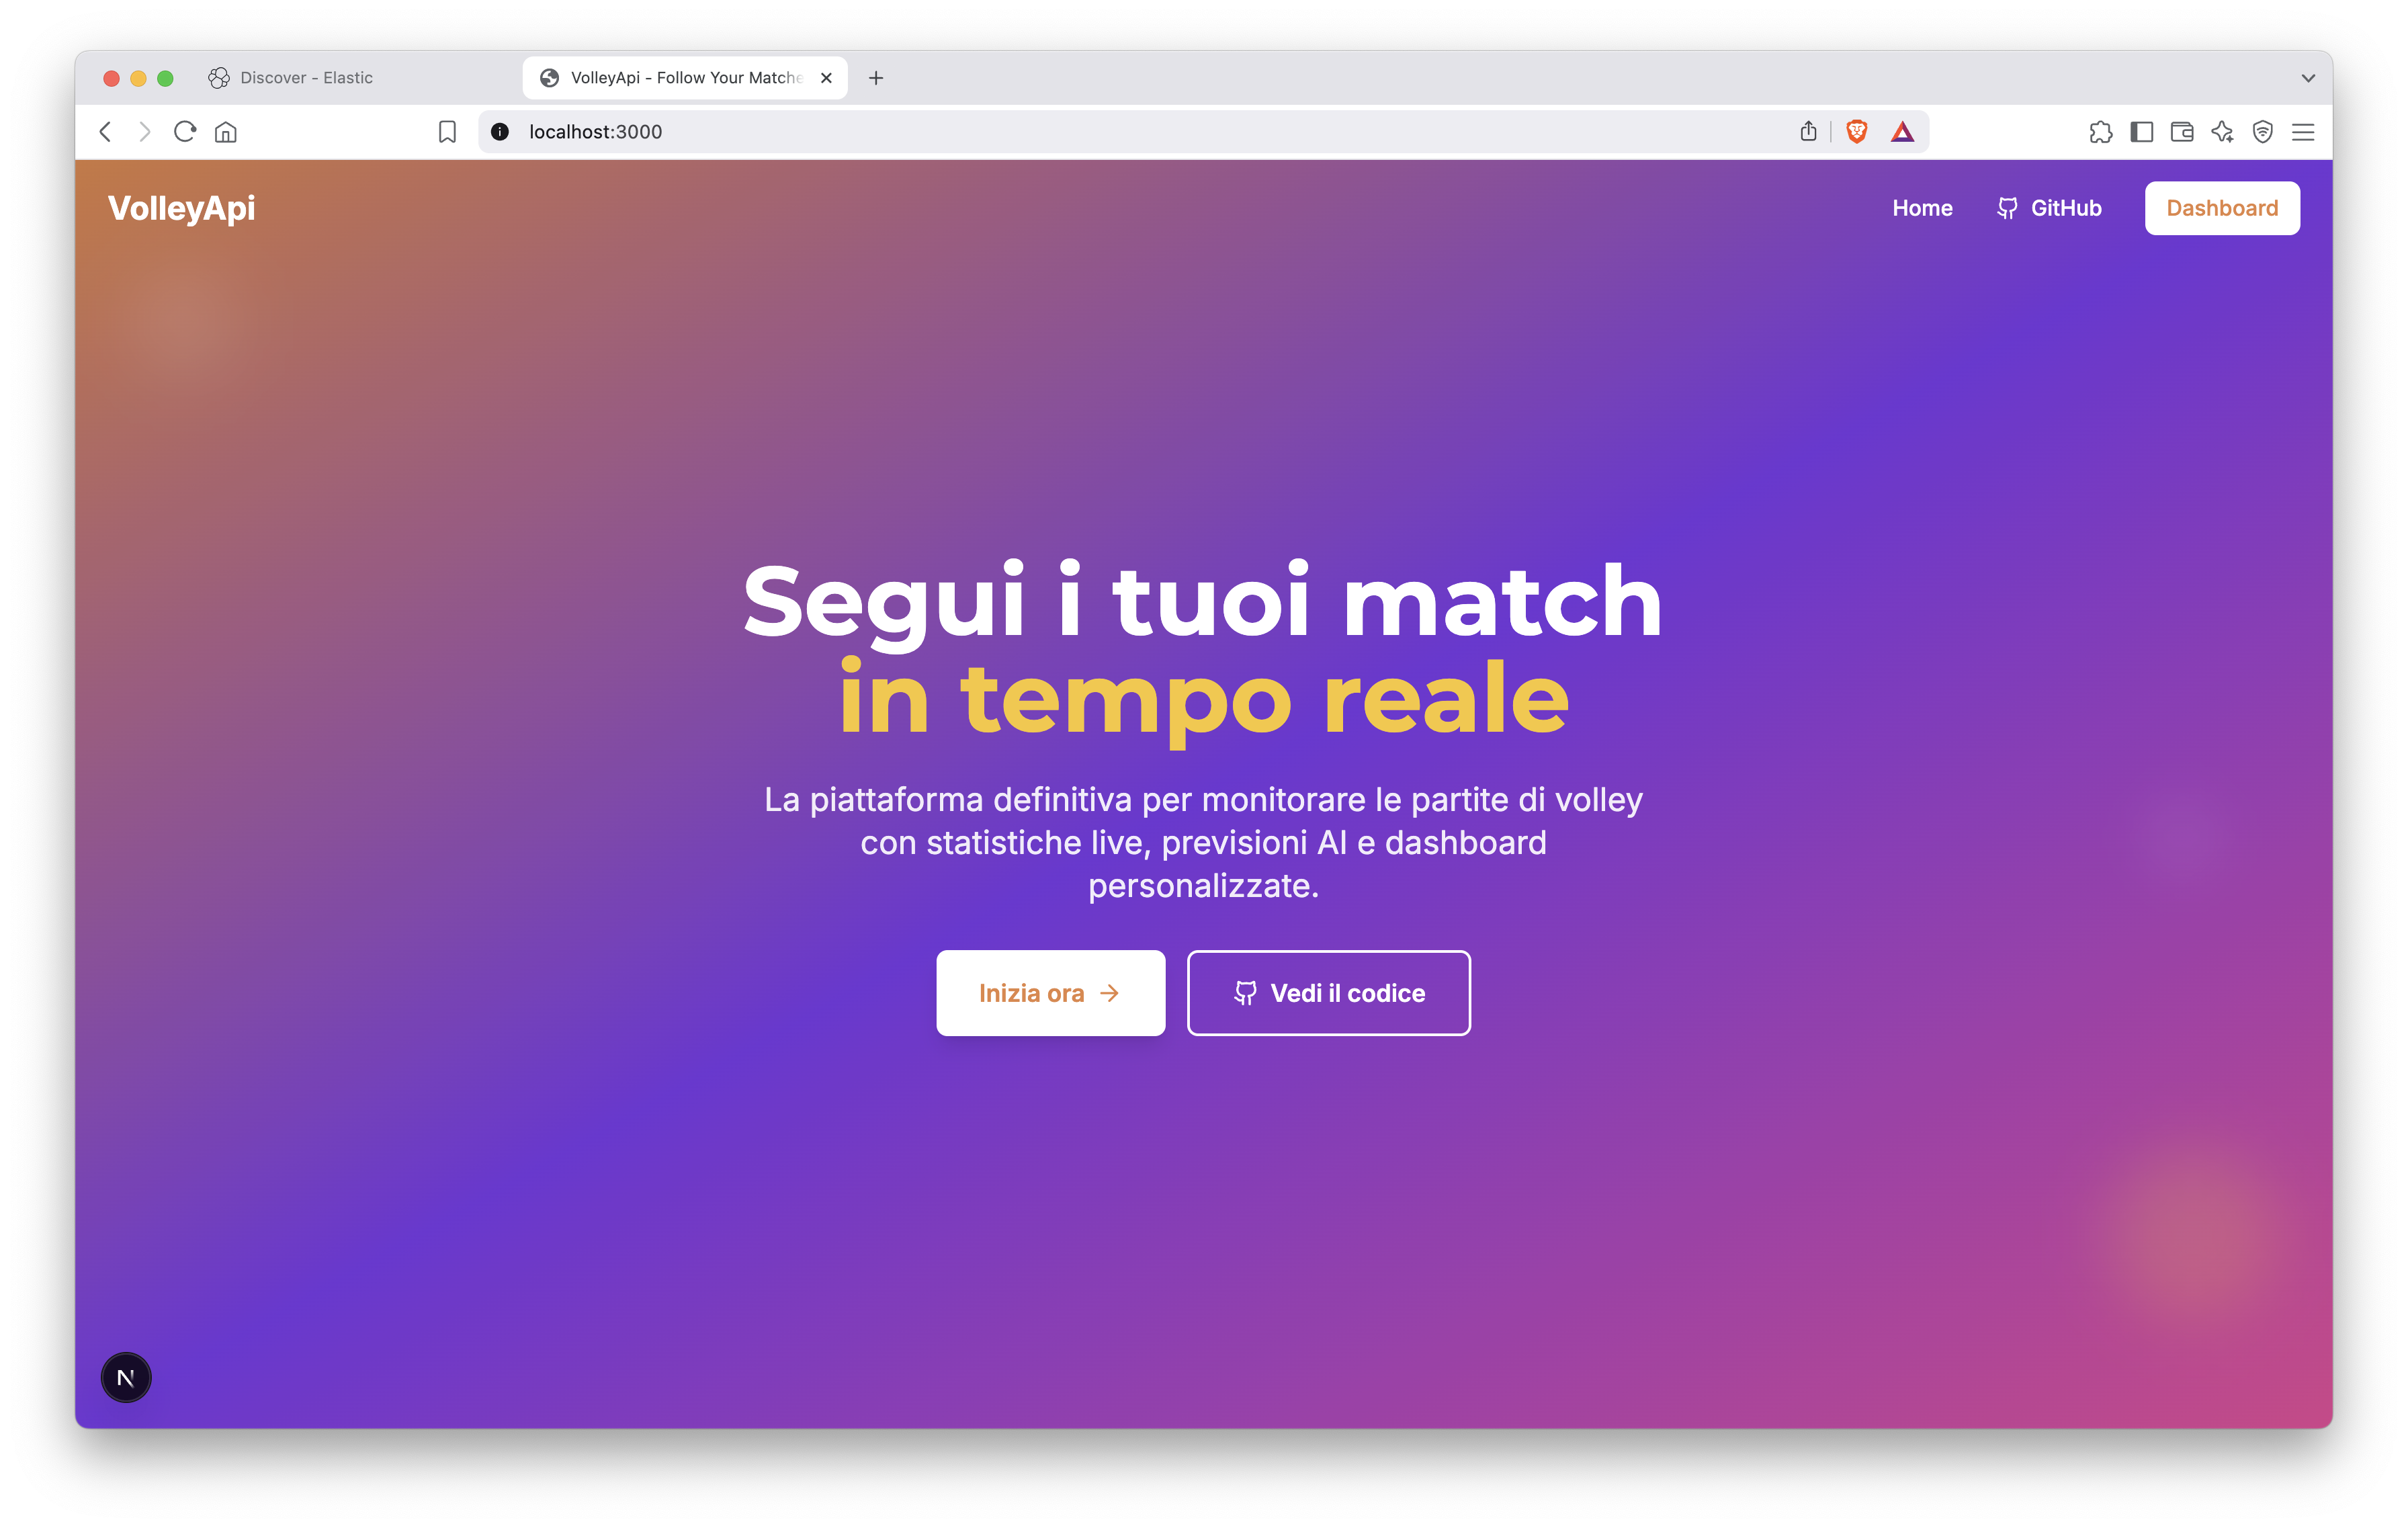
\includegraphics[width=\textwidth]{home.png}
    \label{fig:home web app}
\end{minipage}



L’architettura del progetto segue le convenzioni di Next.js, con una struttura chiara e modulare che facilita l’estensione e la manutenzione del codice : 
\begin{itemize}
    \item \texttt{app/}: definizione delle rotte e delle pagine principali,
    \item \texttt{components/}: insieme di componenti UI riutilizzabili,
    \item \texttt{public/}: risorse statiche come immagini e icone,
    \item \texttt{styles/}: fogli di stile personalizzati tramite Tailwind CSS,
    \item \texttt{utils/}: funzioni di utilità condivise tra i vari componenti.
\end{itemize}

Il \textit{backend} si trova nella directory \texttt{/backend} ed è sviluppato con \textit{FastAPI}, fornendo un'interfaccia REST che consente al frontend di interrogare Elasticsearch:
\begin{itemize}
    \item \texttt{main.py}: entrypoint dell’applicazione,
    \item \texttt{models/}: definizione dei modelli dati e delle classi di risposta.
\end{itemize}


\section{Backend API: Connessione tra Elasticsearch e Frontend}

Il backend del sistema VolleyLive è sviluppato in \textbf{FastAPI}, una libreria moderna e performante per la costruzione di API RESTful. Il suo ruolo principale è fornire un’interfaccia leggera tra il frontend e il database Elasticsearch, restituendo dati aggiornati in formato JSON da visualizzare nella dashboard.

Nel file \texttt{main.py}, situato nella directory \texttt{/backend}, viene inizializzata l’applicazione FastAPI e viene definita la connessione al servizio Elasticsearch, indirizzato al container \texttt{elasticsearch-volley}. La comunicazione avviene tramite richieste HTTP POST, con payload in formato JSON.

La funzione centrale del backend è \texttt{es\_search(payload: dict)}, che incapsula la logica di invio delle richieste verso Elasticsearch e la gestione degli errori. Essa viene invocata dagli endpoint definiti nell’applicazione, come ad esempio:

\begin{lstlisting}[language=Python]
@app.get("/match/{match_id}")
def get_match_data(match_id: int):
    query = {
        "query": { "term": { "match_id": match_id } },
        "sort": [ { "timestamp": { "order": "desc" } } ],
        "size": 1
    }
    result = es_search(query)
    hits = result.get("hits", {}).get("hits", [])

    if not hits:
        raise HTTPException(status_code=404, detail="Match non trovato")

    return hits[0]["_source"]
\end{lstlisting}

Questo endpoint consente di ottenere l’\textit{ultimo snapshot disponibile per una determinata partita}, identificata tramite \texttt{match\_id}. Il risultato restituito contiene i dati completi della partita, tra cui punteggi, stato, set vinti e lo score predittivo \texttt{predicted\_win}.
\\

Il secondo endpoint, definito con

\begin{lstlisting}[language=Python]
@app.get("/matches/{match_id}/sets-predictions")
\end{lstlisting}

recupera invece l’intera sequenza di aggiornamenti per una data partita, ordinando i documenti per \texttt{timestamp} in ordine crescente. Dopo il fetch, il backend suddivide i risultati in due array distinti: \texttt{sets}, contenente gli oggetti \texttt{set\_info} con relativo \texttt{timestamp}, e \texttt{predictions}, con i valori \texttt{predicted\_win} e i rispettivi \texttt{timestamp}.


In fase di sviluppo, il middleware CORS è configurato per accettare richieste da qualsiasi origine, permettendo la comunicazione con il frontend anche in ambienti locali.

L’interfaccia API così progettata offre un punto di accesso semplice e modulare ai dati, ed è facilmente estendibile per supportare filtri aggiuntivi, endpoint aggregati o sistemi di caching futuri.


\section{Struttura e Funzionalità della Dashboard}

\noindent\begin{minipage}{\textwidth}
  \centering
  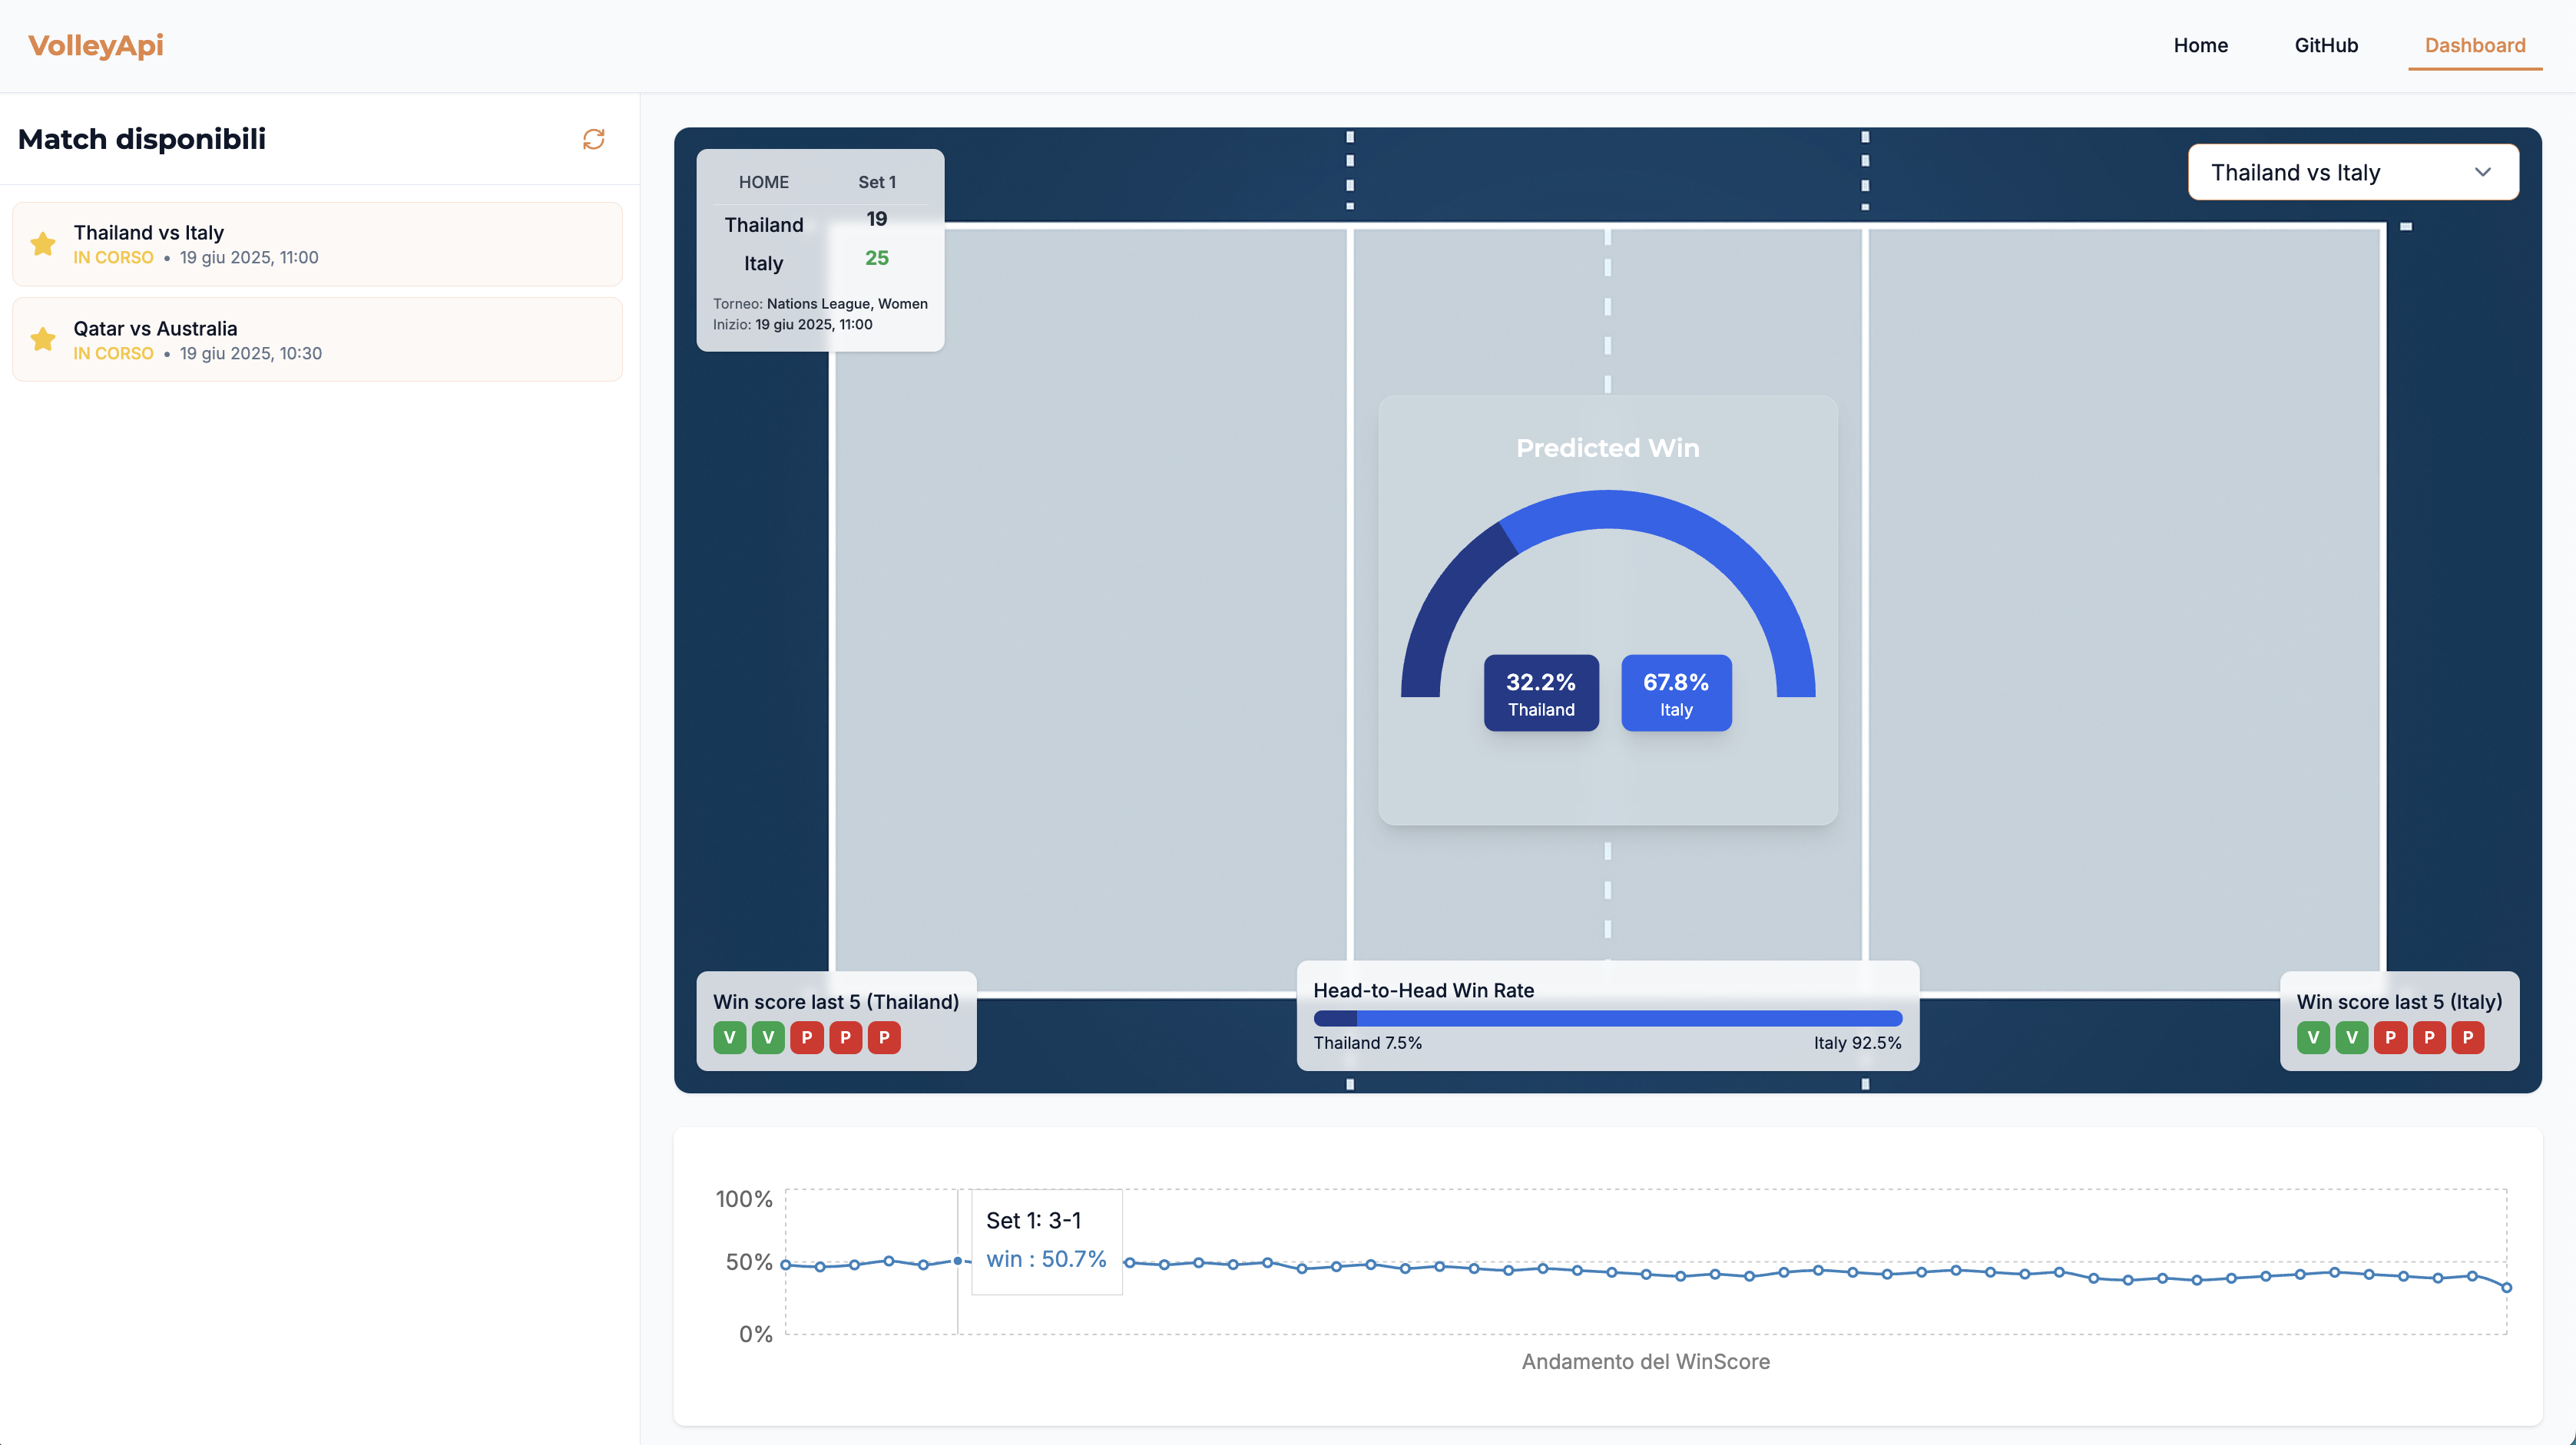
\includegraphics[width=\textwidth]{dashboard.png}
  \label{fig:dashboard}
\end{minipage}

\\
\\
La dashboard del sistema VolleyLive è progettata per fornire una panoramica completa e interattiva delle partite in corso, aggiornandosi in tempo reale tramite le API interne. L’interfaccia si compone principalmente di due sezioni: una colonna laterale sinistra per la selezione dei match e un’area centrale che visualizza i dettagli del match attivo.

Nella colonna sinistra vengono elencate le partite disponibili, con informazioni essenziali come i nomi delle squadre, lo stato della partita (\textit{``in corso''}) e l’orario d’inizio. Ogni riga è selezionabile e l’utente può anche marcare un match come preferito tramite l’icona a forma di stella. La lista si aggiorna dinamicamente interrogando l’API di backend, mostrando solo i match attualmente live.

La sezione principale della dashboard mostra nel dettaglio le informazioni della partita selezionata. In alto a sinistra è presente un box riassuntivo con:
\begin{itemize}
  \item i nomi delle due squadre,
  \item i punteggi aggiornati set per set,
  \item il torneo e l’orario della partita.
\end{itemize}

Al centro dello schermo viene visualizzato il valore di \textbf{predicted win}, ovvero la probabilità stimata di vittoria calcolata dal modello di machine learning. Questo valore è rappresentato tramite un grafico a semicerchio (gauge) che mostra in modo chiaro l’andamento della probabilità tra squadra di casa e ospite.

Nella parte inferiore della schermata sono presenti tre blocchi distinti:
\begin{itemize}
  \item A sinistra, una sintesi della forma recente della squadra di casa, con gli ultimi cinque risultati (vittorie e sconfitte) rappresentati da pallini colorati.
  \item Al centro, una barra che rappresenta le statistiche degli scontri diretti (\textit{head-to-head win rate}) tra le due squadre, utile per contestualizzare la previsione.
  \item A destra, lo stesso indicatore di forma per la squadra ospite.
\end{itemize}

Infine, nella parte più bassa viene mostrato un grafico a linea che rappresenta l’\textbf{andamento temporale del punteggio predittivo}. Questo consente all’utente di osservare come si è evoluta la probabilità di vittoria nel corso del match, fornendo una visione più profonda sull’equilibrio o sul dominio tra le squadre.

Tutti i dati sono aggiornati automaticamente ogni pochi secondi, senza necessità di refresh manuale. Grazie a questo meccanismo di aggiornamento continuo, l’utente può seguire in tempo reale l’evoluzione della partita, con un’interfaccia chiara, responsiva e focalizzata sugli elementi più rilevanti.




% ===============================
% CAPITOLO 5 - Risultati
% ===============================

\chapter{Esecuzione del Sistema e Risultati Osservati}

\section{Esecuzione Completa della Pipeline}

Per comprendere il funzionamento del sistema VolleyLive, è utile seguire passo per passo il percorso di un dato all'interno della pipeline, partendo dal momento in cui viene generato dallo script Python fino alla sua comparsa nel frontend. Questo paragrafo illustra un esempio concreto, utilizzando log e snapshot effettivamente raccolti durante una sessione di monitoraggio reale.
Ai fini della chiarezza espositiva, vengono mostrate solo le componenti principali della pipeline di analisi in tempo reale (producer, Kafka, Spark, Elasticsearch e Frontend), omettendo Logstash, il backend API e strumenti di ispezione come Kibana, poiché non influenzano direttamente il flusso dati trattato in questa sezione dimostrativa.

\subsection*{Snapshot in Ingresso}

\noindent\begin{minipage}{\textwidth}
  \centering
    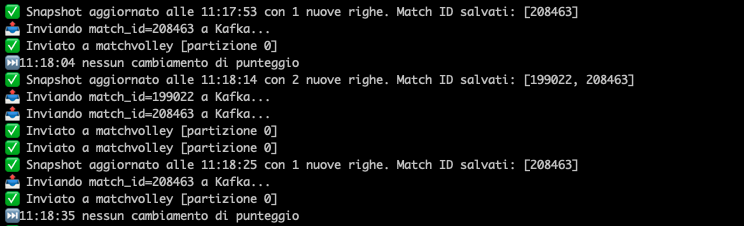
\includegraphics[width=\textwidth]{producer.png}
    \label{fig:producer.py}
\end{minipage}
Il producer Python esegue interrogazioni periodiche all’API SportDevs e genera uno o più snapshot ogni 10 secondi. In un caso osservato, l’aggiornamento delle partite con match ID 199022 e 208463 viene rilevato alle ore 11:18:14 e i dati vengono immediatamente inviati al topic Kafka \texttt{matchvolley}.


\subsection*{Invio su Kafka}
Ogni snapshot viene pubblicato nel topic Kafka dedicato, nella partizione 0. Il terminale conferma l’avvenuto invio per ciascun match, specificando il timestamp e il numero di righe aggiornate. Le righe riportate, come visibile nel dump CSV, contengono il x\texttt{match\_id}, il timestamp, lo stato dei set, punteggi parziali e diverse feature derivate, tra cui \texttt{set\_diff}, \texttt{score\_diff} e \texttt{predicted\_win}.


\noindent\begin{minipage}{\textwidth}
  \centering
    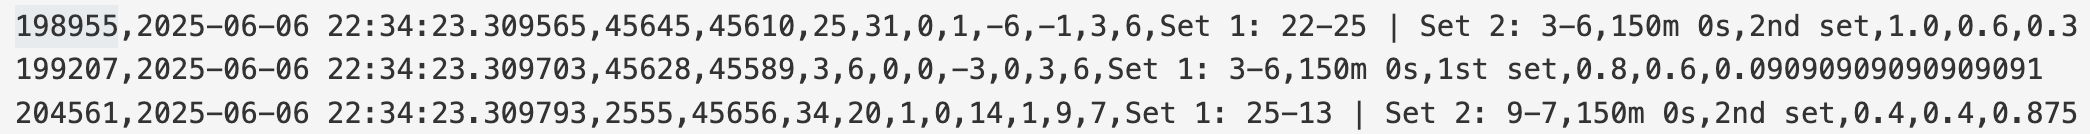
\includegraphics[width=\textwidth]{snapshoat.png}
    \label{fig:dati grezzi}
\end{minipage}

\subsection*{Elaborazione con Spark}
Il micro-batch di Spark intercetta i nuovi offset da Kafka, elabora il contenuto e applica il modello predittivo. Dai log si osserva che Spark riceve il messaggio (es. offset da 1626 a 1627), esegue le trasformazioni e calcola lo score predittivo tramite regressione logistica. L'intero batch viene processato in meno di un secondo (con un tempo di \texttt{triggerExecution} pari a 978\,ms), e i risultati vengono immediatamente scritti nell’indice \texttt{volleyball\_matches}.

\subsection*{Scrittura su Elasticsearch}
Dopo l'elaborazione, i documenti vengono scritti in Elasticsearch attraverso il connettore Spark--ES. I log riportano le operazioni di scrittura e i commit all’interno della directory di checkpoint \texttt{/tmp/spark-es-logreg-checkpoint}, a conferma della persistenza dei dati. La scrittura avviene in modalità \texttt{append}, mantenendo lo storico degli snapshot nel tempo.

\subsection*{Visualizzazione sul Frontend}
Infine, il frontend interroga l’indice Elasticsearch tramite il backend API, ottenendo i documenti aggiornati. 

\noindent\begin{minipage}{\textwidth}
  \centering
    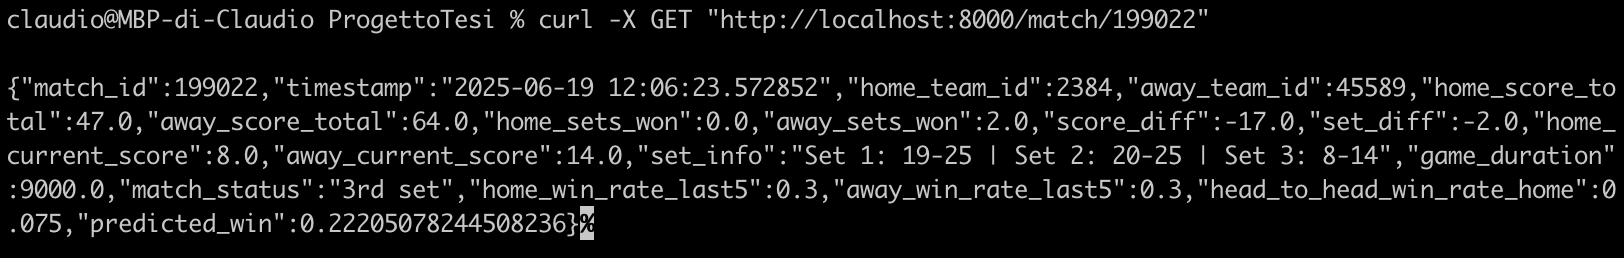
\includegraphics[width=\textwidth]{API.png}
    \label{fig:API REST}
\end{minipage}

La dashboard mostra in tempo reale lo stato della partita, il punteggio set per set e la probabilità di vittoria (\texttt{predicted\_win}) calcolata pochi secondi prima da Spark.

\noindent\begin{minipage}{\textwidth}
  \centering
    \includegraphics[width=\textwidth]{dashboard2.png}
    \label{fig:dashboard}
\end{minipage}

\section{Valutazione del Modello Predittivo}

Per misurare la capacità di generalizzazione del modello, i dati sono stati suddivisi per \texttt{match\_id}: il 80\,\% degli snapshot è stato utilizzato per l’addestramento, mentre il restante 20\,\% è stato riservato al test, garantendo l’assenza di leak tra train e test.

Sul test set, costituito da 721 snapshot, si ottengono le seguenti metriche:

\begin{itemize}
  \item \textbf{Accuracy:} 0.7462 \\
    Il modello classifica correttamente circa 3 snapshot su 4.
  \item \textbf{AUC–ROC:} 0.8479 \\
    Buon potere discriminante tra vittoria e sconfitta, indipendente dalla soglia di decisione.
  \item \textbf{Log Loss:} 0.5764 \\
    Indica la qualità delle probabilità predette; valori più bassi denotano migliore calibrazione.
  \item \textbf{Brier Score:} 0.1939 \\
    Misura la distanza quadratica tra probabilità predetta e risultato osservato.
\end{itemize}

\noindent La matrice di confusione sul test set è:

\begin{verbatim}
              Pred=0   Pred=1
Actual=0       328       117
Actual=1        66       210
\end{verbatim}

Si riscontrano 117 falsi positivi e 66 falsi negativi, a indicare situazioni in cui il modello sovrastima o sottostima la probabilità di vittoria.

\medskip

\noindent Va inoltre ricordato che il file \texttt{trainer\_model.csv} è in continua crescita: ogni nuovo snapshot arricchisce il dataset e consente un costante miglioramento delle prestazioni del modello. Con l’aumentare dei dati raccolti, è ragionevole attendersi un incremento dell’AUC–ROC e una diminuzione di Log Loss e Brier Score.

\medskip

\noindent Nel paragrafo seguente confronteremo queste prestazioni con l’evoluzione predittiva di un singolo match, analizzando come varia lo \textit{score} predittivo in corrispondenza dei momenti chiave della partita.



\section{ Caso Studio: Evoluzione di un Match}


Per valutare il comportamento dinamico del modello predittivo durante lo svolgimento di una partita, sono stati analizzati due incontri particolarmente significativi (ID 199023 e 198981), identificati all’interno del dataset sulla base dell’ampiezza delle oscillazioni predittive e della lunghezza del match.

\subsection*{Fase iniziale}

Nel primo match (ID 199023), la probabilità iniziale di vittoria per la squadra di casa era pari a 0{,}30, un valore piuttosto basso. Tale previsione rifletteva correttamente le condizioni di partenza: la squadra ospite presentava infatti una percentuale di vittorie nelle ultime cinque partite pari a 0{,}8, contro lo 0{,}2 della squadra di casa, e uno storico di scontri diretti sfavorevole. Analogamente, nel secondo match (ID 198981), il valore iniziale di \texttt{predicted\_win} per la squadra di casa era intorno a 0{,}32, anche in questo caso coerente con i dati storici sfavorevoli.

\subsection*{Fase intermedia}

Nel corso del primo set del match 199023, il punteggio si è mantenuto bilanciato fino al 13–13, momento in cui la probabilità stimata oscillava tra 0{,}31 e 0{,}33. Tuttavia, una breve serie negativa ha portato la squadra di casa a 13–16, facendo scendere la previsione a 0{,}28, segno della sensibilità del modello anche a brevi break sfavorevoli.

Nel match 198981, invece, si è osservato un andamento più instabile nella fase centrale: tra il secondo e il terzo set, il punteggio ha visto alternarsi situazioni di parità e vantaggio da entrambe le parti. La \texttt{predicted\_win}, inizialmente scesa fino a 0{,}25 dopo un primo set perso, è risalita fino a 0{,}44 in corrispondenza di una rimonta nel secondo parziale, dimostrando la reattività del modello ai cambi di trend.

\subsection*{Fase finale}

Nel match 199023, il punteggio complessivo ha raggiunto 2–2 in set, portando le squadre al tie-break. In questa fase, la \texttt{predicted\_win} ha mostrato le oscillazioni più marcate, con picchi fino a 0{,}58 per la squadra di casa durante un parziale di vantaggio nel set decisivo. Tuttavia, anche piccole inversioni nel punteggio hanno prodotto rapide fluttuazioni predittive, confermando che la fase finale del match è percepita dal modello come altamente incerta.

Anche nel match 198981 la partita si è conclusa al tie-break, con l’ultima porzione della curva predittiva che ha oscillato in modo più irregolare. La probabilità ha raggiunto un valore massimo di 0{,}55 per la squadra di casa, prima di scendere bruscamente negli ultimi snapshot, segnalando la progressiva definizione dell’esito sfavorevole.

\subsection*{Partita a senso unico: stabilità predittiva}

A titolo di confronto, è stato analizzato anche un match conclusosi con un risultato netto di 3–1 a favore della squadra di casa (match ID 199009). In questo caso, l’andamento della \texttt{predicted\_win} ha mostrato un comportamento molto più stabile: partendo da un valore iniziale di 0{,}51, è cresciuta progressivamente fino a 0{,}67 senza subire inversioni significative. La bassa escursione predittiva (delta = 0{,}16) riflette l’assenza di ribaltamenti o fasi di incertezza, confermando che il modello riesce a mantenere coerenza in situazioni di chiara supremazia.



\noindent\begin{minipage}{\textwidth}
  \centering
    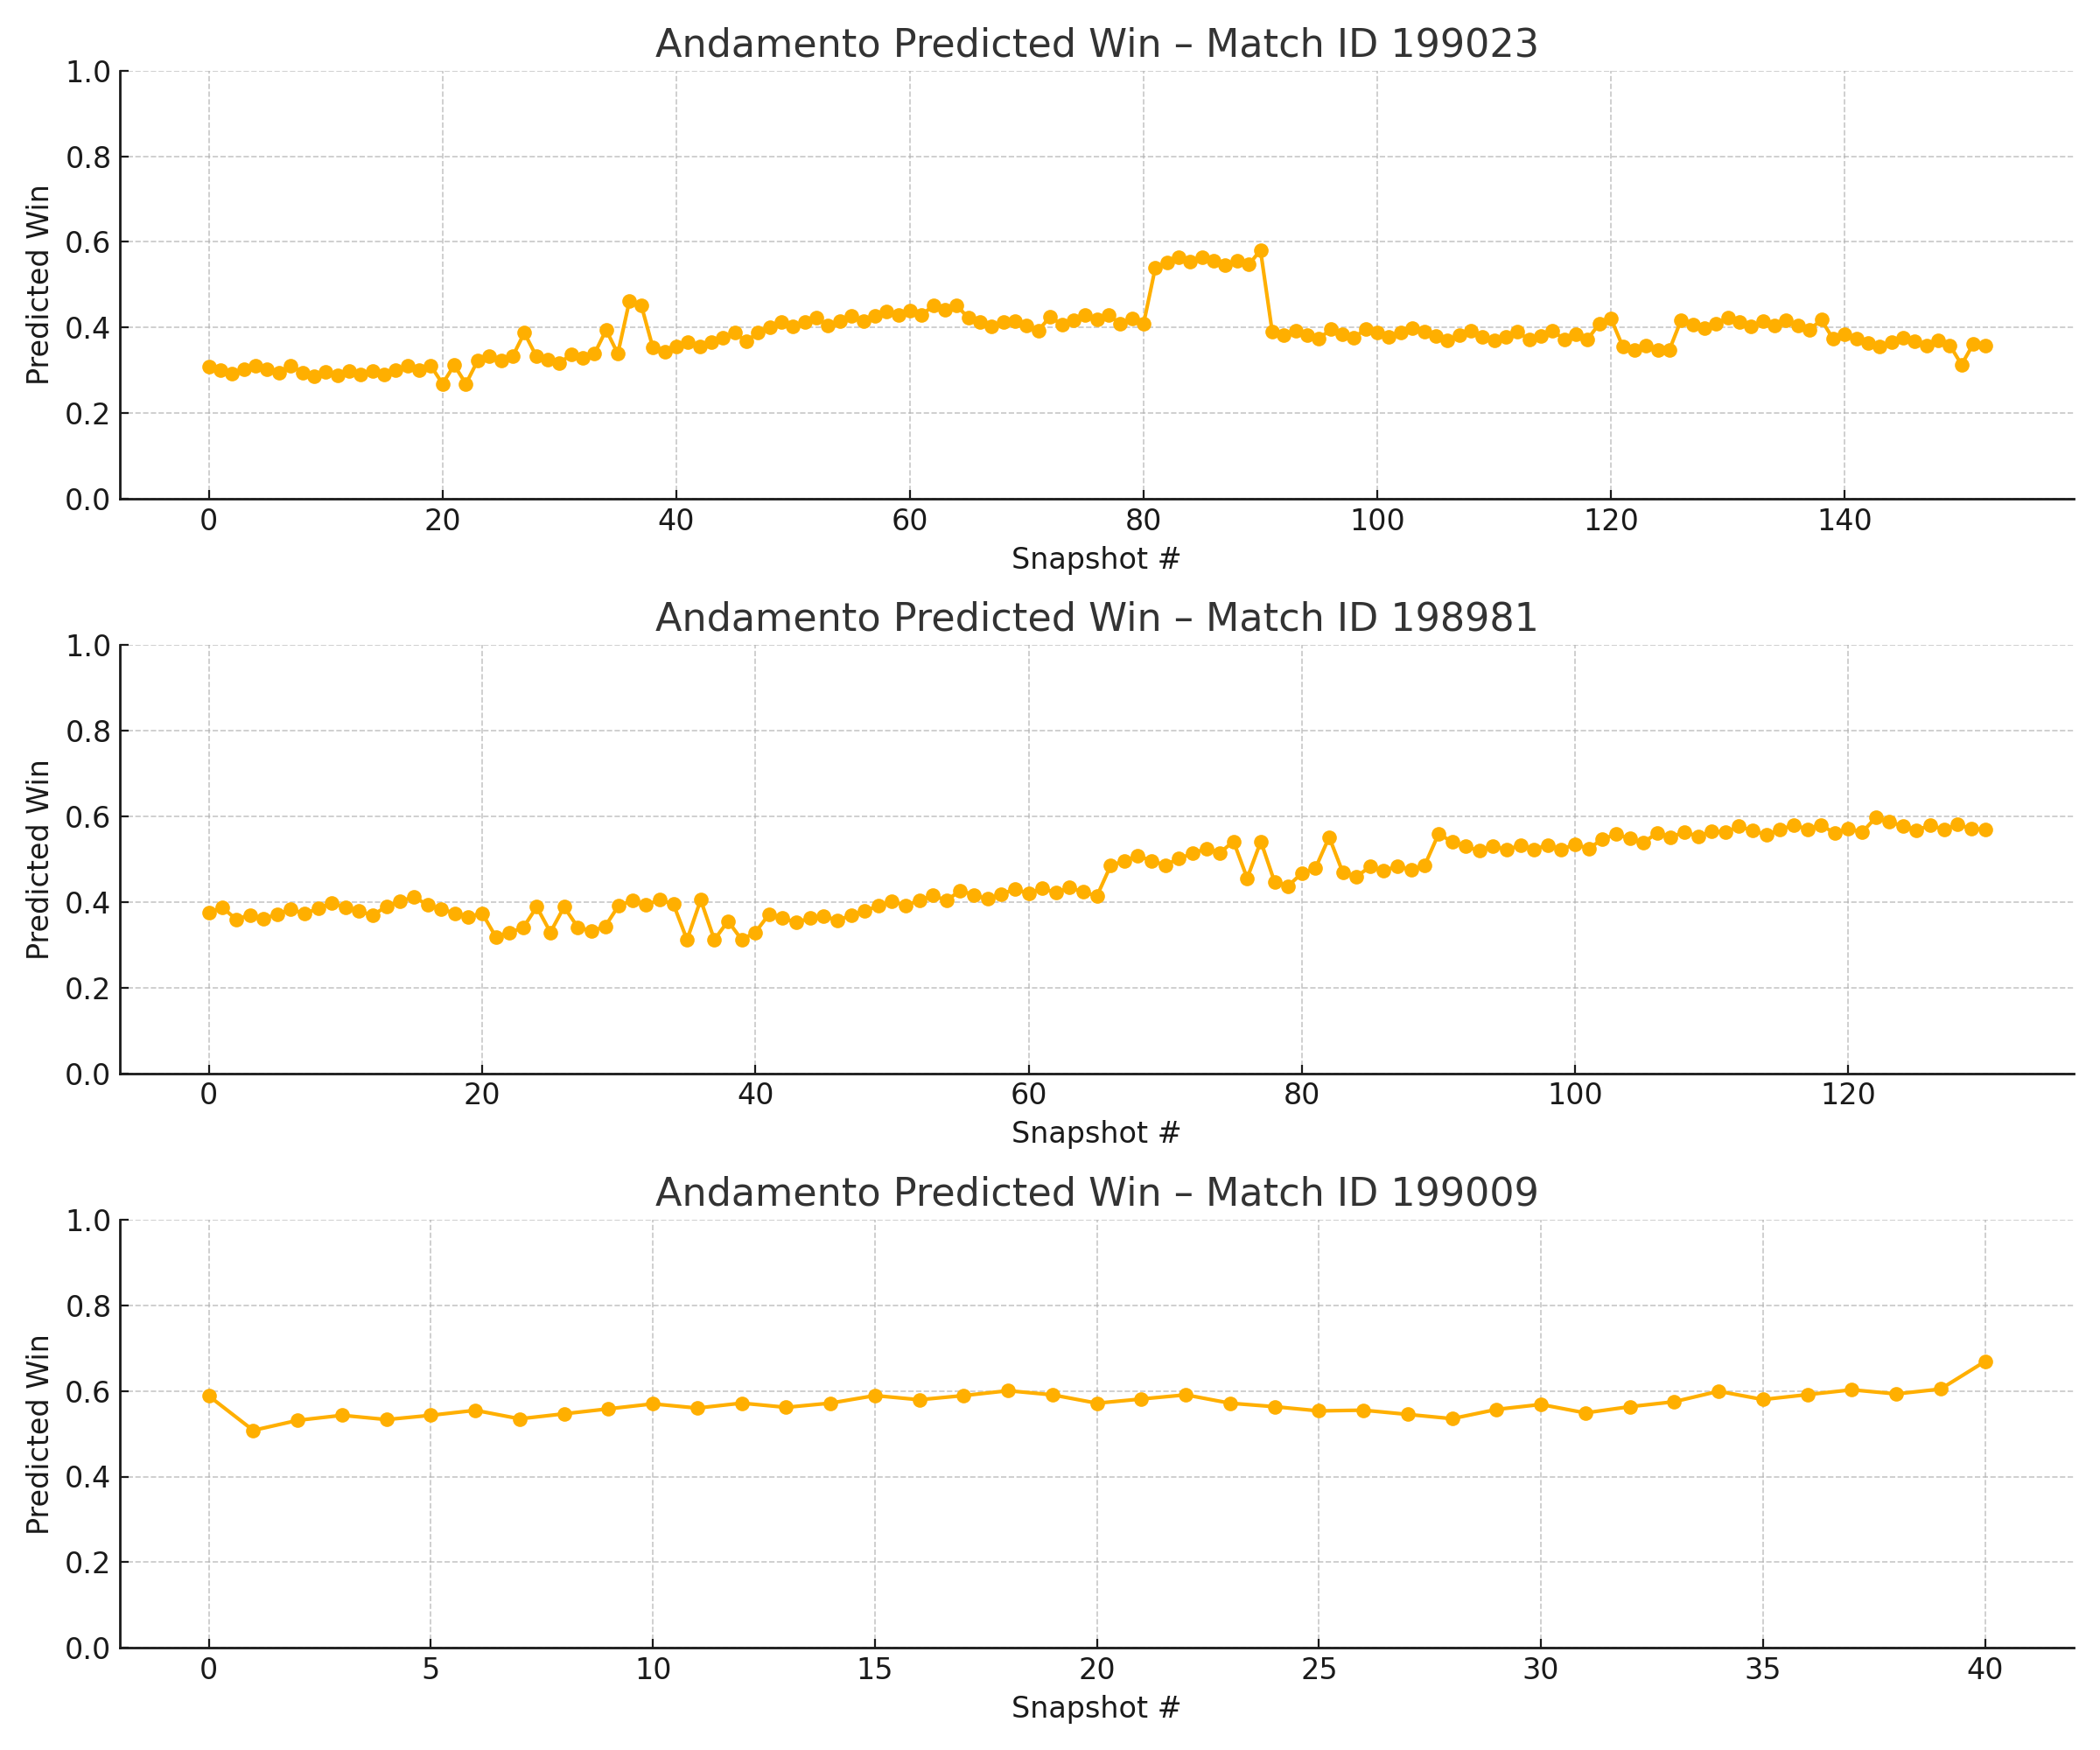
\includegraphics[width=\textwidth]{andamento_predicted_win_match_simple_x.png}
    \label{fig:andamento-predicted-win}
\end{minipage}


\section{Latenza e Prestazioni della Pipeline}

Uno degli obiettivi principali del progetto VolleyLive è garantire la reattività del sistema in tempo quasi reale. A tal fine, è stata progettata una pipeline in grado di elaborare, analizzare e rendere disponibili i dati entro pochi secondi dal loro arrivo.

La misura della latenza è stata effettuata tracciando il tempo intercorrente tra la generazione di uno snapshot live da parte del producer Python (punto di partenza) e la visualizzazione aggiornata sul frontend (punto di arrivo). A ogni snapshot è associato un campo \texttt{timestamp}, che permette di confrontare i tempi intermedi nei vari passaggi della pipeline.

Dalle osservazioni sperimentali condotte su partite reali, la latenza complessiva è risultata mediamente compresa tra \textbf{3 e 6 secondi}, con picchi massimi occasionali fino a 10 secondi nei casi di maggiore congestione. La suddivisione approssimativa della latenza può essere così schematizzata:

\begin{itemize}
  \item \textbf{Producer → Kafka → Logstash:} meno di 1 secondo;
  \item \textbf{Logstash → Spark (elaborazione micro-batch):} circa 1--2 secondi;
  \item \textbf{Spark → Elasticsearch (scrittura):} circa 1 secondo;
  \item \textbf{Elasticsearch → API → Frontend:} circa 1--2 secondi.
\end{itemize}

La scelta di utilizzare una pipeline always-on e un modello predittivo snello (regressione logistica) ha permesso di mantenere bassi i tempi di elaborazione, senza rinunciare all’arricchimento degli snapshot con feature derivate e score predittivo.

L’uso di checkpoint su Spark e la persistenza continua su Elasticsearch garantiscono inoltre la tolleranza ai guasti e il recupero in caso di restart del sistema, contribuendo alla robustezza complessiva dell’architettura.


% ===============================
% CAPITOLO 6 - Conclusioni
% ===============================

\chapter*{Conclusioni e Sviluppi Futuri}

Il progetto \textit{VolleyLive} ha dimostrato come sia possibile realizzare una pipeline di analisi in tempo reale basata su tecnologie open source, in grado di raccogliere, elaborare e visualizzare dati dinamici relativi a partite di pallavolo in corso. L’integrazione tra strumenti come Kafka, Spark ed Elasticsearch ha permesso non solo la gestione efficiente del flusso informativo, ma anche l’implementazione di un primo livello di analisi predittiva applicata al contesto sportivo.

L’intero sistema è stato progettato con una struttura modulare e scalabile: ogni componente (dalla raccolta dati al frontend) può essere esteso o sostituito senza compromettere l’integrità dell’architettura. Questo approccio ha favorito la sperimentazione di modelli di machine learning integrabili all’interno della pipeline, con l’obiettivo di stimare in tempo reale la probabilità di vittoria durante lo svolgimento di una partita.

Le analisi presentate nel Capitolo~\ref{cap:risultati}, condotte su match reali, hanno mostrato la capacità del modello di adattarsi al contesto della gara, rispondendo con sensibilità ai cambiamenti nel punteggio. Sebbene l’accuratezza del modello sia ancora soggetta alla quantità e alla qualità dei dati raccolti, i risultati ottenuti evidenziano la solidità della struttura implementata e la validità dell’approccio adottato.

È importante sottolineare alcuni limiti attuali del sistema, legati principalmente alla natura delle fonti dati. Le informazioni raccolte tramite l’API di SportDevs, pur essendo sufficientemente ricche per le analisi svolte, non costituiscono una fonte ufficiale federale, e possono contenere errori, discrepanze o aggiornamenti ritardati. Inoltre, alcune partite vengono restituite in modo incompleto o con frequenza irregolare, introducendo una certa discontinuità nella raccolta degli snapshot.

Nonostante questi vincoli, \textit{VolleyLive} rappresenta una base concreta su cui costruire future estensioni: tra queste, l’integrazione di analisi più avanzate basate su dati storici aggregati, il confronto tra competizioni diverse, e l’arricchimento dell’interfaccia utente con funzionalità predittive interattive.


\end{document}
